\chapter{Results}

This chapter presents the results of the project in a structured way to evaluate whether a proof of concept has been successfully achieved and to explore the applicability of modern \gls{dl} architectures for testing \gls{db} \gls{sw}. The chapter is divided into two main sections, each corresponding to a key phase of the project.

The first section discusses the results from the model training process. This includes an overview of the generated output graphs and a discussion of the model performance in terms of accuracy, loss, and generalization capabilities.

The second section focuses on the results obtained from integrating the complete system. It covers how the \gls{hil} was used to change the \gls{db} views, trigger the Flask application and execute the image analysis process. The final detection results are reviewed and used to assess the system overall functionality and reliability.

\section{Model Training Results}
This section demonstrates how well the model learned to detect the telltale icons of the KTM \gls{db}. It begins with a brief summary of the training setup and continues with an analysis of the results.

As the project is intended to operate on real camera images rather than high-quality Photoshop exports, it was essential to ensure that the model did not overfit on the prepared \gls{ds}. To evaluate this, the model was trained for five, twenty, and fifty epochs, and the resulting loss curves were compared. This comparison aimed to verify that the training process maintained good generalization and did not show signs of overfitting.

Among the different evaluation metrics, the most important during training was the class loss. This metric indicates how accurately the model learned to classify the telltale icons during both the training and validation phases. The class loss trends for the three training durations are shown in Figure~\ref{fig:E_Comparison}.

\begin{figure}[!ht]
    \centering
    \begin{subfigure}[b]{0.65\textwidth}
        \centering
        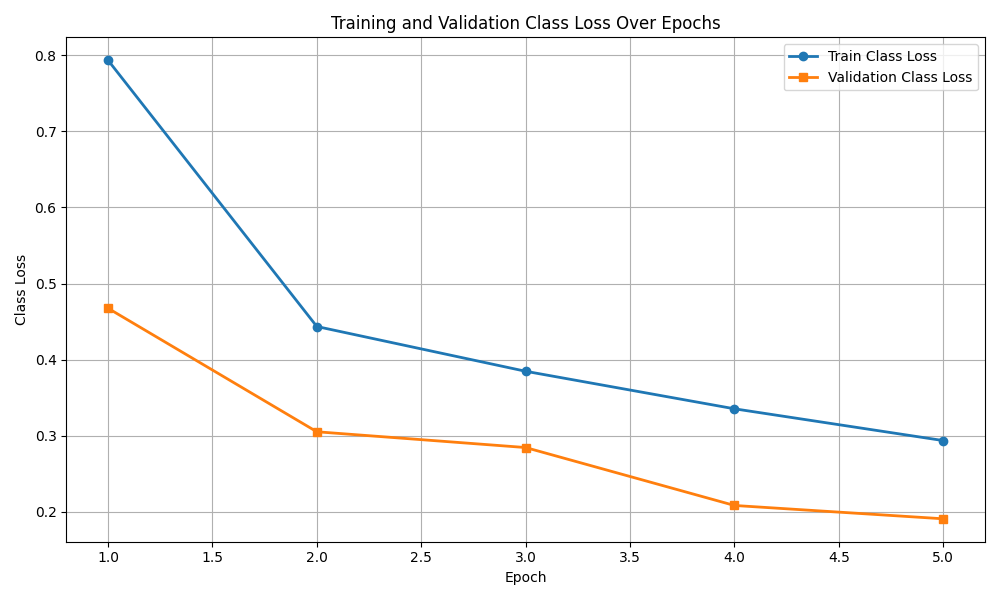
\includegraphics[width=\textwidth]{Figures/Results/Graphs/5_Epochs/class_loss_plot.png}
        \caption{Five epochs.}
        \label{fig:5_E}
    \end{subfigure}

    \vskip 0.5cm
    % Second subfigure
    \begin{subfigure}[b]{0.65\textwidth}
        \centering
        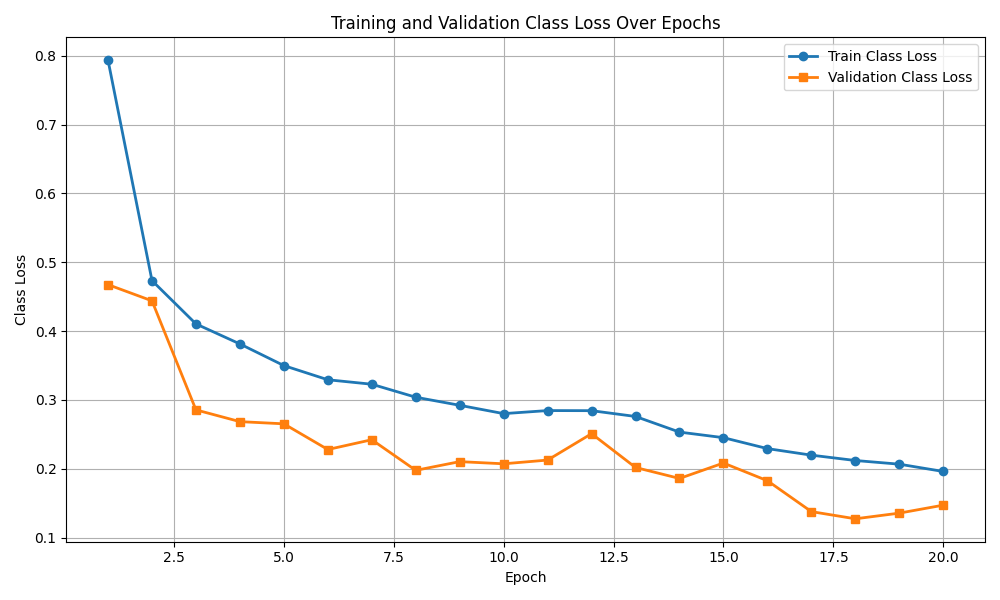
\includegraphics[width=\textwidth]{Figures/Results/Graphs/20_Epochs/class_loss_plot.png}
        \caption{Twenty epochs.}
        \label{fig:20_E}
    \end{subfigure}
    
    \vskip 0.5cm
    % Second subfigure
    \begin{subfigure}[b]{0.65\textwidth}
        \centering
        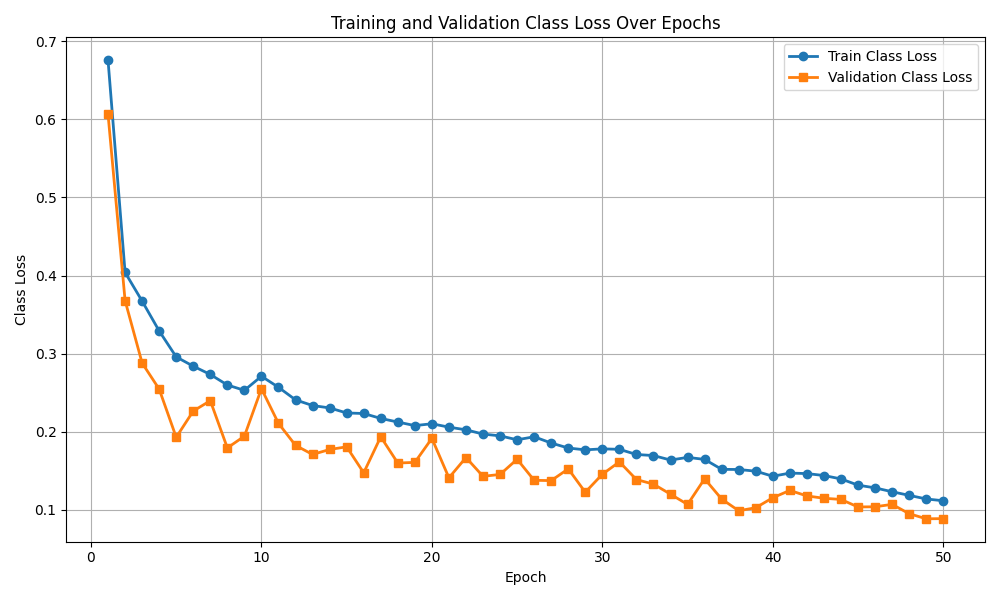
\includegraphics[width=\textwidth]{Figures/Results/Graphs/50_Epochs/class_loss_plot.png}
        \caption{Fifty epochs}
        \label{fig:50_E}
    \end{subfigure}
    
    \caption{Comparison of class loss curves for training and validation after five, twenty, and fifty epochs. These results help assess whether the model overfits on the \gls{ds} and how well it generalizes to unseen data.}
    \label{fig:E_Comparison}
\end{figure}

The model showed consistent improvement as the number of training epochs increases. In the five epoch plot, the training and validation class loss decrease steadily but are still relatively high, indicating that the model has not yet fully converged. However, with twenty epochs, the loss values are significantly lower and the validation loss stays close to the training loss. This behaviour suggests that the model is learning effectively without overfitting.

In the fifty epoch plot, the training loss continues to decrease gradually, and the validation loss shows small fluctuations while maintaining a downward trend. This behavior suggests that the model is generalizing well, even over longer training durations. The absence of a sharp rise in validation loss confirms that overfitting did not occur. However, the absence of improvements over a period of ten epochs and a value of validation loss of 0.08856 indicate that the model is performing as required and further training might lead to better perforance on the Photoshop files but not on the camera images. Overall, the fifty epochs model offers the best balance between learning and generalization.

The model was further validated on the test \gls{ds} to assess its performance under realistic conditions. To ensure that the model would generalize well to actual input data, twenty camera images were manually captured, annotated and included in the test \gls{ds}. This increased the total test set to one hundred fifteen images

Figure~\ref{fig:conf_matrix} presents the confusion matrix generated after running the model on this test set. Each row represents the predicted class, while each column represents the ground truth. The diagonal values indicate correctly classified instances and off-diagonal values would represent misclassifications. As shown, the model was able to accurately detect all ten telltale classes with high accuracy. All confusion matrix values are concentrated along the diagonal, with no misclassifications observed. This results confirm that the model performs consistently across all target classes. Additionally, Figure~\ref{fig:Sample_CI} shows an example of a camera image where all telltale icons were correctly detected with high confidence, each exceeding ninety percent.

\begin{figure}[!ht]
    \centering
    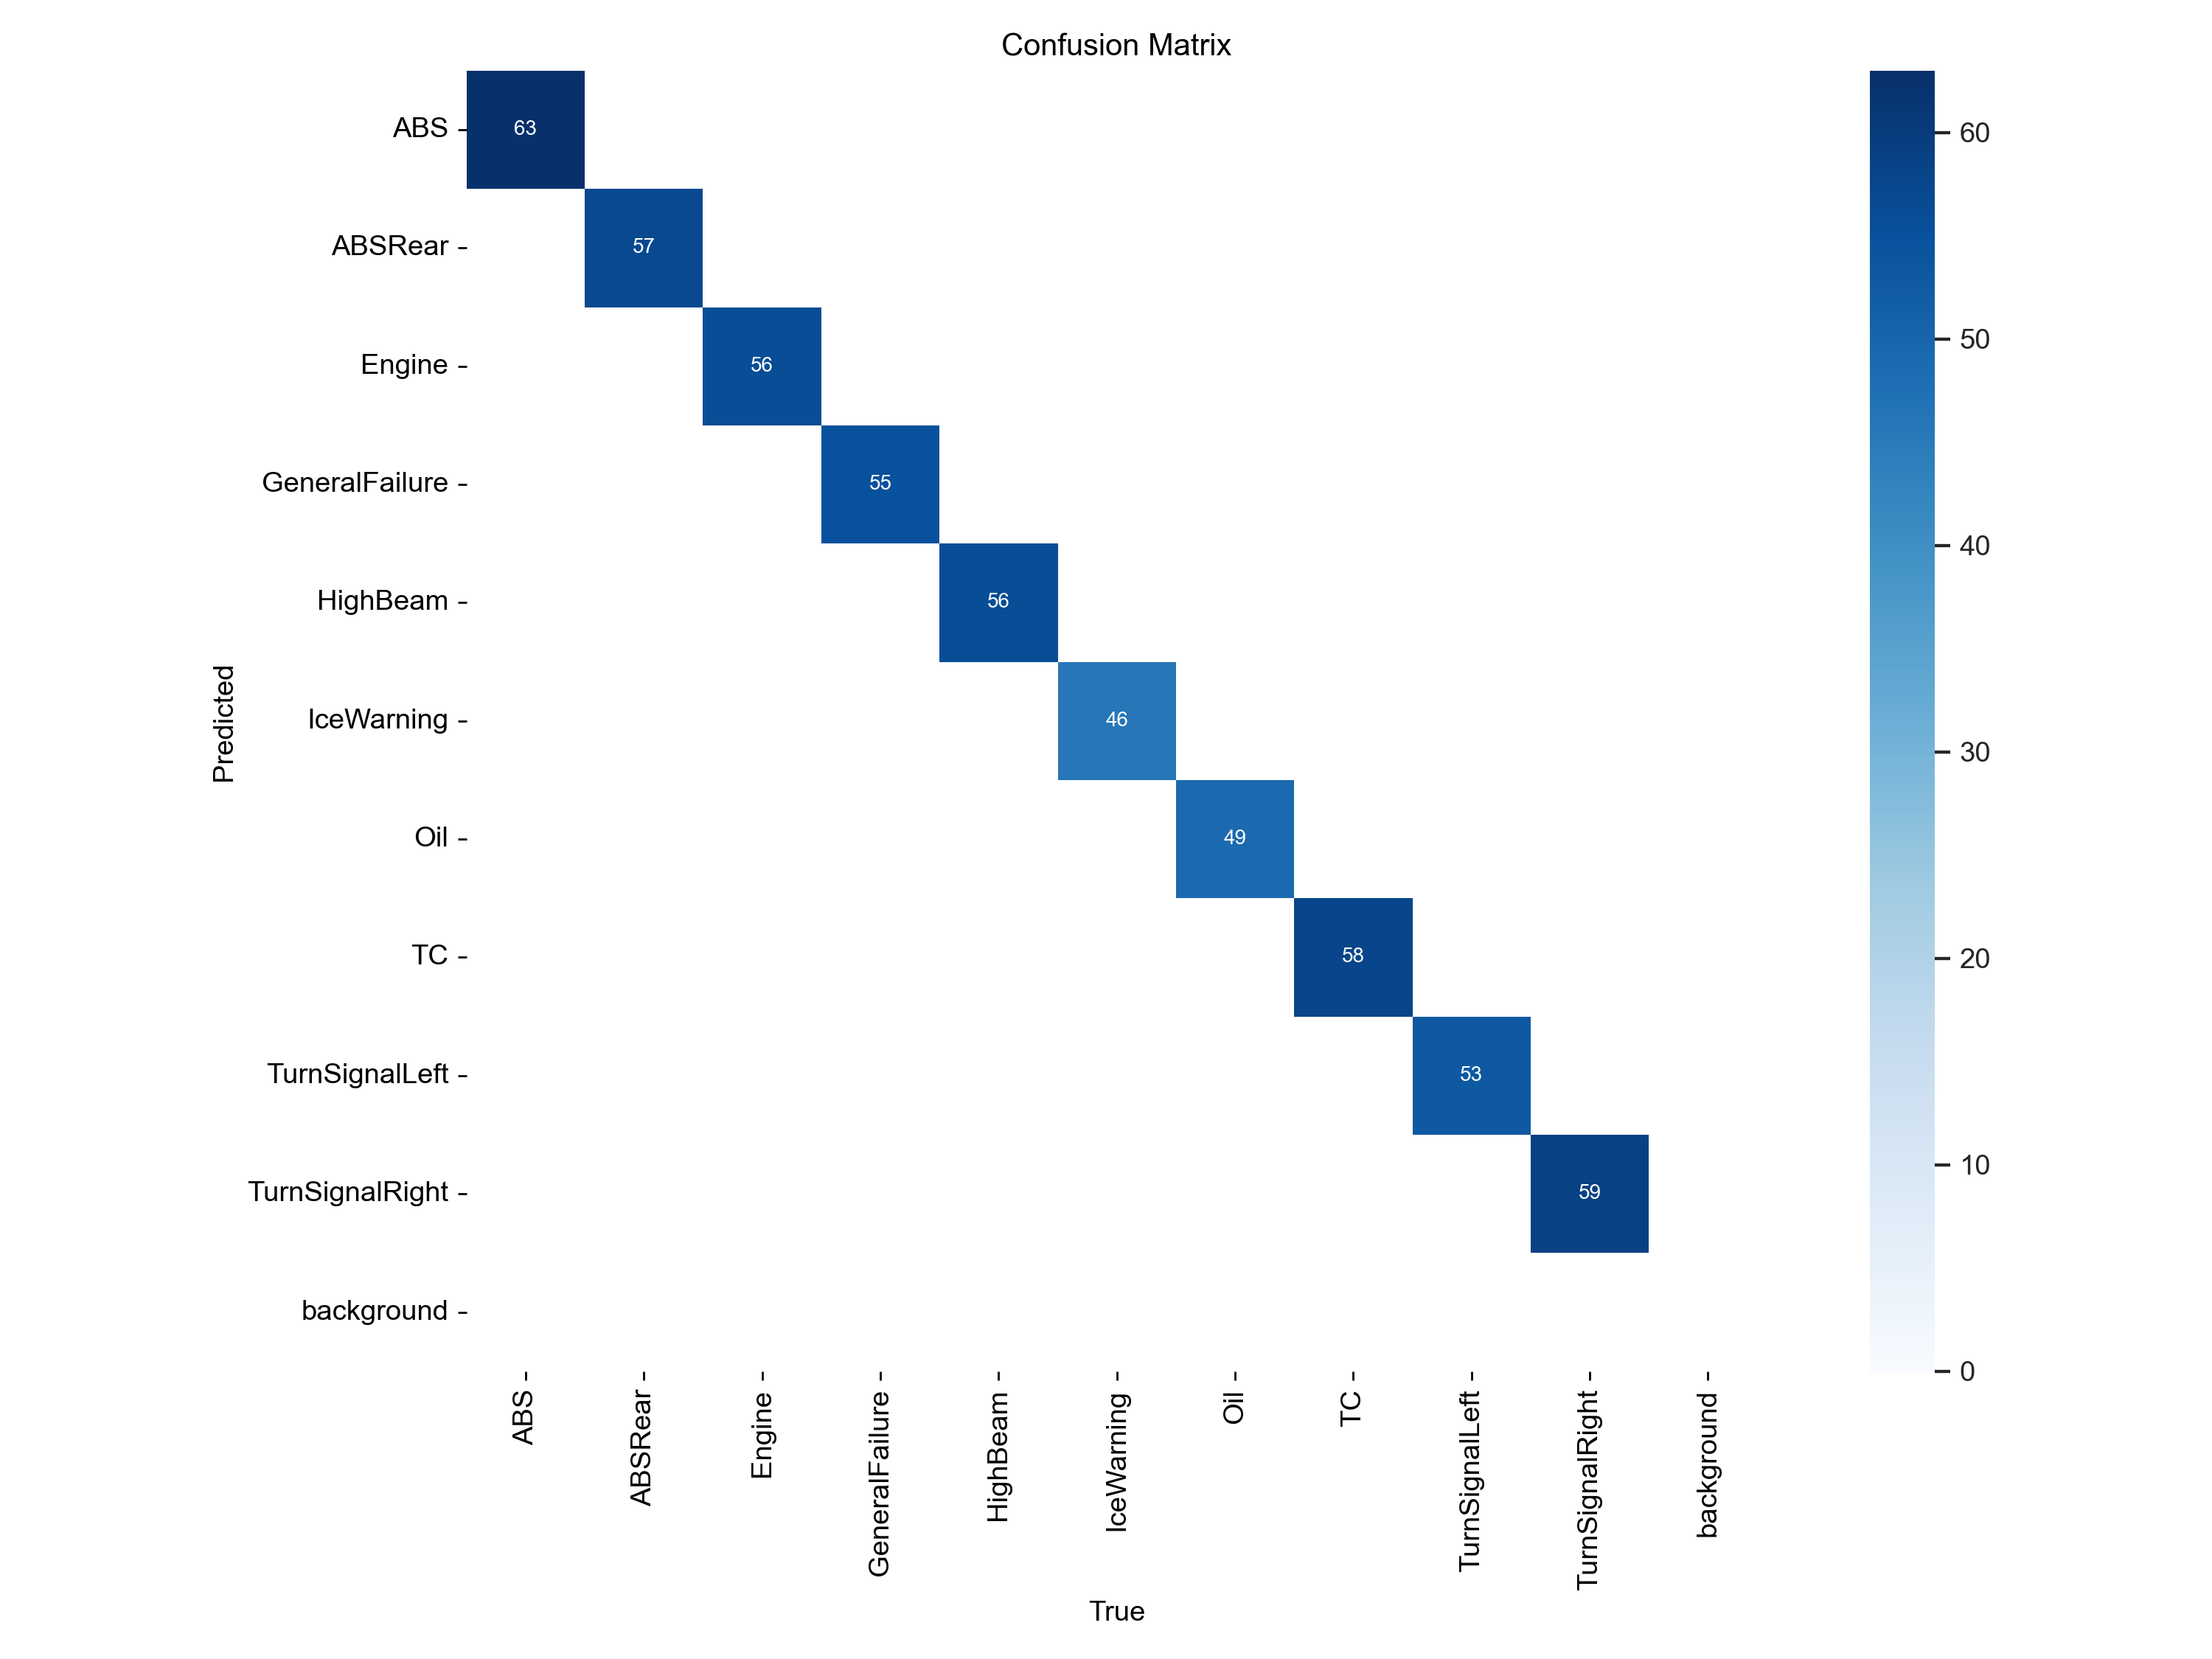
\includegraphics[width=1\textwidth]{Figures/Results/Graphs/Test/confusion_matrix.png}
    \caption{Confusion matrix showing the classification performance on the full test \gls{ds} including twenty real camera images.}
    \label{fig:conf_matrix}
\end{figure}


\begin{figure}[!ht]
    \centering
    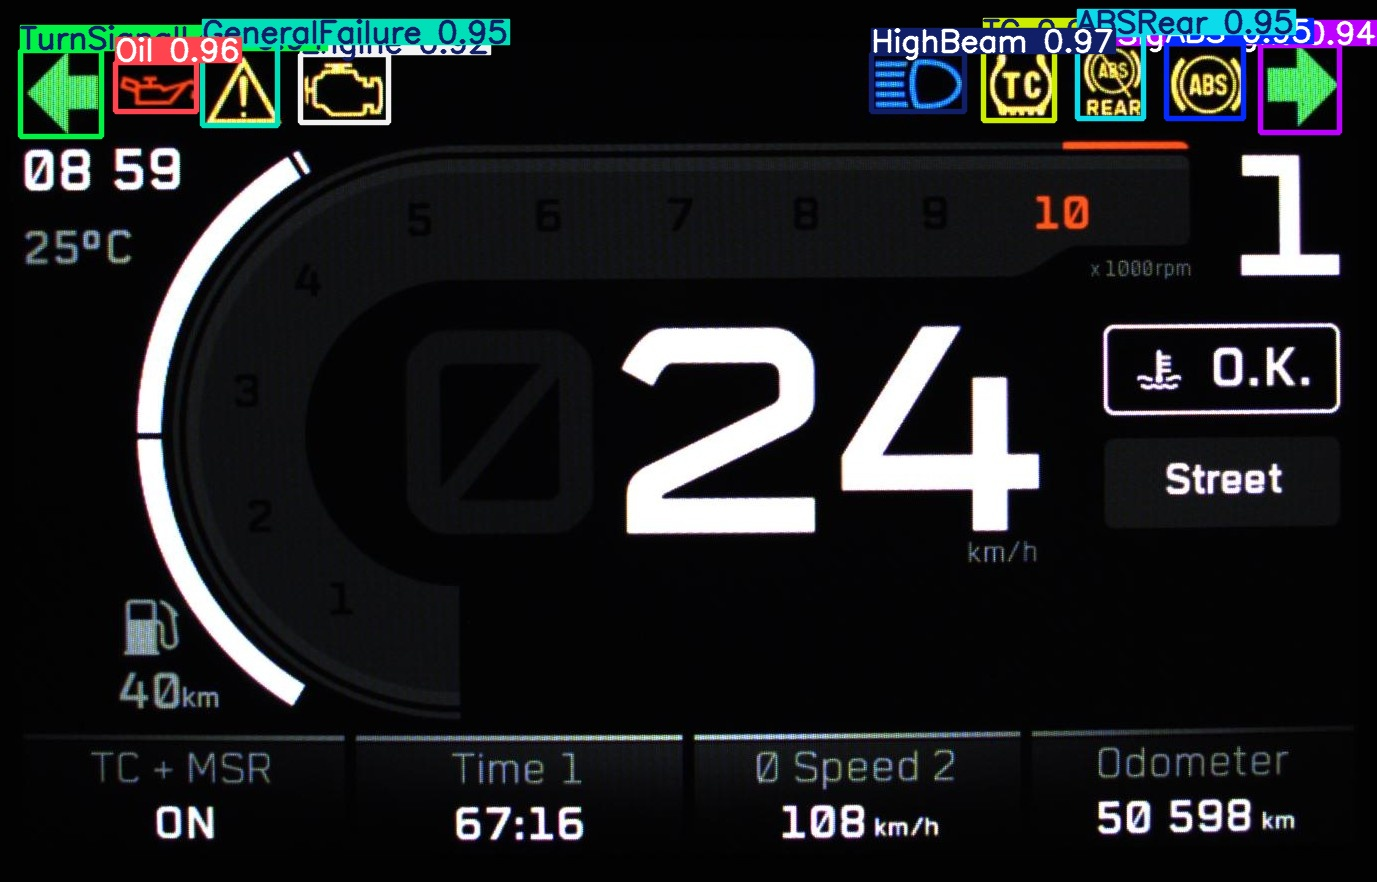
\includegraphics[width=0.8\textwidth]{Figures/Results/Graphs/Test/8_bmp.rf.8110c0e7d7a1723405054135cabc6cbf.jpg}
    \caption{Sample inference result on a real camera image, showing correct detection of all telltale icons with confidence scores above ninety percent.}
    \label{fig:Sample_CI}
\end{figure}

The model demonstrated perfect performance, which is uncommon in the field of \gls{dl}. However, given the simplicity of the task, the use of a high quality and custom made \gls{ds} with perfectly balanced classes, appropriate augmentation techniques, a high resolution \gls{cs} and a controlled lighting environment, such results are considered reasonable and expected.


\section{System Integration Results}
